\documentclass[12pt]{article}

\usepackage[a4paper,margin=1in]{geometry}
\usepackage{amsmath,amssymb}
\usepackage{newtxtext,newtxmath} % Times-style font
\usepackage{fancyhdr}
\usepackage{listings}
\usepackage{graphicx}
\usepackage{float}
\usepackage{algorithm}
\usepackage{algpseudocode}
\usepackage{xcolor}
\usepackage{booktabs}
\usepackage{array}

\setlength{\textfloatsep}{10pt}
\setlength{\floatsep}{10pt}

\setlength{\parindent}{0pt}
\setlength{\parskip}{5pt}

% Keep entire document at 12 pt
\AtBeginDocument{
    \fontsize{12pt}{14pt}\selectfont
}

\lstdefinestyle{code}{
    language=Python,
    basicstyle=\ttfamily\fontsize{10pt}{12pt}\selectfont,
    breaklines=true,
    breakatwhitespace=false,
    frame=single,
    numbers=left,
    numberstyle=\tiny\color{gray},
    keywordstyle=\color{blue},
    commentstyle=\color{gray},
    stringstyle=\color{green!50!black},
    columns=fullflexible,
    keepspaces=true,
    showstringspaces=false
}

\lstdefinestyle{output}{
    basicstyle=\ttfamily\fontsize{10pt}{12pt}\selectfont,
    breaklines=true,
    breakatwhitespace=false,
    frame=single,
    numbers=none,
    backgroundcolor=\color{gray!4},
    columns=fullflexible,
    keepspaces=true,
    showstringspaces=false
}

% ------------------------------------------------
% Header
% ------------------------------------------------

\pagestyle{fancy}
\fancyhf{}

\fancyhead[L]{Name: Kishan Sahu{\hspace{4cm}}}
\fancyhead[R]{Enrollment No.: P26DS017}

\renewcommand{\headrulewidth}{0.4pt}
\setlength{\headheight}{15pt}

\begin{document}

% ------------------------------------------------
% TITLE
% ------------------------------------------------

\begin{center}
\textbf{Computer Science and Engineering Department, SVNIT, Surat}\\
\textbf{M.Tech. I -- Semester I}\\
\textbf{Design and Analysis of Algorithm (CSDS103)}\\
\textbf{Lab Assignment: Comprehensive Algorithmic Analysis}\\
\textbf{Lab Assignment 7: String Matching Algorithms}
\end{center}
\vspace{-4pt}
\hrule
\vspace{4pt}

\vspace{0.3cm}

\section{Introduction and Objectives}
The string matching problem consists of finding all occurrences of a given pattern string $P$ of length $m$ within a text string $T$ of length $n$ ($m \le n$). Both strings are constructed from an alphabet $\Sigma$. A pattern $P$ is said to occur with shift $s$ ($0 \le s \le n - m$) if:
\begin{equation}
T[s + j] = P[j] \quad \text{for all } 0 \le j \le m - 1
\end{equation}

This laboratory report implements, analyzes, and empirically benchmarks three classical string matching paradigms:
\begin{enumerate}
    \item \textbf{Naive String Matching}: Direct sliding window without preprocessing.
    \item \textbf{Knuth--Morris--Pratt (KMP)}: Preprocessing of $P$ using the Longest Proper Prefix which is also Suffix (LPS) array to prevent redundant character backtracking.
    \item \textbf{Rabin--Karp}: Rolling hash matching with character verification upon hash equivalence.
\end{enumerate}

All implementations are coded from scratch in standard Python without relying on built-in substring search primitives (such as \texttt{in} or \texttt{str.find()}).

% =========================================================================
% PROBLEM 1
% =========================================================================
\section{Problem 1: Naive String Matching Algorithm}

\subsection{Theoretical Formulation and Complexity}
The Naive algorithm examines every possible shift $s \in [0, n - m]$ sequentially. For each shift, it performs character-by-character comparisons between $T[s \dots s+m-1]$ and $P[0 \dots m-1]$. As soon as a mismatch is detected, the search for the current shift terminates, and the pattern shifts rightward by 1 position ($s \leftarrow s + 1$).

\begin{itemize}
    \item \textbf{Best-Case Time Complexity}: $\mathcal{O}(n)$. Occurs when the very first character $P[0]$ fails to match $T[s]$ across all shifts, resulting in exactly 1 comparison per shift: $(n - m + 1) \times 1 = \mathcal{O}(n)$.
    \item \textbf{Worst-Case Time Complexity}: $\mathcal{O}((n - m + 1) \cdot m)$. Occurs when all characters match up to the $(m-1)$-th position and mismatch at the last character (or when every position matches completely), forcing $m$ comparisons for each of the $n - m + 1$ shifts.
    \item \textbf{Auxiliary Space Complexity}: $\mathcal{O}(1)$. Only loop indices and comparison counters are maintained.
\end{itemize}

\subsection{Python Implementation}
\begin{lstlisting}[style=code, caption={Naive String Matching Implementation}]
def naive_string_match(text, pattern):
    """
    Performs Naive String Matching without built-in functions.
    Returns:
        occurrences (list): 0-indexed starting positions of matches.
        comparisons (int): Total character comparisons performed.
    """
    n = len(text)
    m = len(pattern)
    occurrences = []
    comparisons = 0

    if m == 0 or m > n:
        return occurrences, comparisons

    for i in range(n - m + 1):
        match = True
        for j in range(m):
            comparisons += 1
            if text[i + j] != pattern[j]:
                match = False
                break
        if match:
            occurrences.append(i)

    return occurrences, comparisons
\end{lstlisting}

\subsection{Execution and Verification}
The algorithm was tested on the assignment test case:
\begin{center}
$T = \text{"AABAACAADAABAABA"}, \quad P = \text{"AABA"}$
\end{center}

\begin{lstlisting}[style=output, caption={Problem 1 Execution Output on Sample Input}]
--- Problem 1: Basic Test ---
Text    : AABAACAADAABAABA
Pattern : AABA
Pattern found at indices: [0, 9, 12]
Total Character Comparisons: 30
\end{lstlisting}

\subsection{Worst-Case Analysis Demonstration}
To demonstrate the worst-case behavior, we construct an adversarial input where $T$ is a string of 20 identical characters and $P$ has 4 matching characters followed by a mismatching character:
\begin{center}
$T = \text{"AAAAAAAAAAAAAAAAAAAA"} \quad (n = 20), \qquad P = \text{"AAAAB"} \quad (m = 5)$
\end{center}

\begin{lstlisting}[style=code, caption={Worst-Case Input Experiment}]
text_worst = "A" * 20
pattern_worst = "A" * 4 + "B"  # Length m = 5
n_w, m_w = len(text_worst), len(pattern_worst)

pos_worst, comp_worst = naive_string_match(text_worst, pattern_worst)
theoretical_worst = (n_w - m_w + 1) * m_w

print("--- Problem 1: Worst-Case Analysis ---")
print(f"Text    : {text_worst} (n = {n_w})")
print(f"Pattern : {pattern_worst} (m = {m_w})")
print(f"Occurrences found          : {pos_worst}")
print(f"Actual Comparisons Done    : {comp_worst}")
print(f"Theoretical Max (n-m+1)*m  : {theoretical_worst}")
print(f"Does actual reach max?     : {comp_worst == theoretical_worst}")
\end{lstlisting}

\begin{lstlisting}[style=output, caption={Problem 1 Worst-Case Execution Output}]
--- Problem 1: Worst-Case Analysis ---
Text    : AAAAAAAAAAAAAAAAAAAA (n = 20)
Pattern : AAAAB (m = 5)
Occurrences found          : []
Actual Comparisons Done    : 80
Theoretical Max (n-m+1)*m  : 80
Does actual reach max?     : True
\end{lstlisting}

\textbf{Explanation of Repeated Comparisons}:
In the experiment above, for each shift $i \in [0, 15]$, the algorithm compares the first 4 characters successfully ($T[i+j] == P[j] = \text{'A'}$ for $j \in \{0, 1, 2, 3\}$). The mismatch occurs on the 5th character ($T[i+4] = \text{'A'} \neq \text{'B'} = P[4]$).
Because the Naive algorithm has \textbf{no memory of prior character matches}, it discards all 4 matched characters and shifts right by only 1 position ($i \leftarrow i + 1$). At the new shift, it re-compares the same text characters from scratch. This causes redundant repeated comparisons, confirming the $(20 - 5 + 1) \times 5 = 80$ operations.

% =========================================================================
% PROBLEM 2
% =========================================================================
\section{Problem 2: Knuth--Morris--Pratt (KMP) String Matching}

\subsection{Theoretical Formulation and Complexity}
The KMP algorithm eliminates redundant comparisons by preprocessing the pattern $P$ into an array called \textbf{LPS} (Longest Proper Prefix which is also Suffix).
For a pattern $P[0 \dots m-1]$, $\text{LPS}[i]$ represents the length of the longest proper prefix of $P[0 \dots i]$ that is also a suffix of $P[0 \dots i]$.

When a mismatch occurs at $P[j]$ after matching $j$ characters with $T[i]$:
\begin{enumerate}
    \item We know that $P[0 \dots j-1]$ matched $T[i-j \dots i-1]$.
    \item If $j > 0$, the next character to compare against $T[i]$ is $P[\text{LPS}[j-1]]$, thereby advancing the pattern without moving the text pointer $i$ backwards.
    \item If $j = 0$, no prefix matched, so the text pointer simply increments ($i \leftarrow i + 1$).
\end{enumerate}

\begin{itemize}
    \item \textbf{Preprocessing Time}: $\mathcal{O}(m)$ to construct the LPS array.
    \item \textbf{Matching Phase Time}: $\mathcal{O}(n)$ because each character of $T$ is advanced forwards, and the pattern index $j$ drops at most $n$ times via LPS.
    \item \textbf{Total Time Complexity}: $\mathcal{O}(n + m)$.
    \item \textbf{Auxiliary Space Complexity}: $\mathcal{O}(m)$ to store the LPS array.
\end{itemize}

\subsection{Python Implementation}
\begin{lstlisting}[style=code, caption={LPS Array Computation and KMP Search}]
def compute_lps(pattern):
    """
    Constructs the LPS (Longest Proper Prefix which is Suffix) array
    without using any built-in pattern matching functions.
    """
    m = len(pattern)
    lps = [0] * m
    length = 0  # Length of previous longest prefix-suffix
    i = 1

    while i < m:
        if pattern[i] == pattern[length]:
            length += 1
            lps[i] = length
            i += 1
        else:
            if length != 0:
                length = lps[length - 1]
            else:
                lps[i] = 0
                i += 1
    return lps

def kmp_search(text, pattern):
    """
    Performs Knuth-Morris-Pratt (KMP) search.
    Returns:
        occurrences (list): Starting indices of pattern matches.
        comparisons (int): Total character comparisons performed.
    """
    n = len(text)
    m = len(pattern)
    occurrences = []
    comparisons = 0

    if m == 0 or m > n:
        return occurrences, comparisons

    lps = compute_lps(pattern)
    i = 0  # Text index
    j = 0  # Pattern index

    while i < n:
        comparisons += 1
        if text[i] == pattern[j]:
            i += 1
            j += 1

        if j == m:
            occurrences.append(i - j)
            j = lps[j - 1]
        elif i < n and text[i] != pattern[j]:
            if j != 0:
                j = lps[j - 1]
            else:
                i += 1

    return occurrences, comparisons
\end{lstlisting}

\subsection{Execution and Verification}
\subsubsection{LPS Array for Sample Pattern \texttt{"ABABCABAB"}}
As specified in the assignment, we construct and verify the LPS array for pattern $P = \text{"ABABCABAB"}$:

\begin{lstlisting}[style=output, caption={LPS Array Output}]
--- Problem 2: LPS Array Construction ---
Pattern: ABABCABAB
Indices: [0, 1, 2, 3, 4, 5, 6, 7, 8]
Chars  : ['A', 'B', 'A', 'B', 'C', 'A', 'B', 'A', 'B']
LPS    : [0, 0, 1, 2, 0, 1, 2, 3, 4]
\end{lstlisting}

\textbf{LPS Breakdown}:
\begin{itemize}
    \item $i=0$ (\texttt{'A'}): No proper prefix $\implies \text{LPS}[0] = 0$.
    \item $i=1$ (\texttt{"AB"}): Prefixes: \texttt{\{"A"\}}, Suffixes: \texttt{\{"B"\}} $\implies \text{LPS}[1] = 0$.
    \item $i=2$ (\texttt{"ABA"}): Proper prefix \texttt{"A"} matches suffix \texttt{"A"} $\implies \text{LPS}[2] = 1$.
    \item $i=3$ (\texttt{"ABAB"}): Proper prefix \texttt{"AB"} matches suffix \texttt{"AB"} $\implies \text{LPS}[3] = 2$.
    \item $i=4$ (\texttt{"ABABC"}): Character \texttt{'C'} breaks suffix matching $\implies \text{LPS}[4] = 0$.
    \item $i=5 \dots 8$: Suffixes matching prefixes build back up: \texttt{"A"} (1), \texttt{"AB"} (2), \texttt{"ABA"} (3), \texttt{"ABAB"} (4).
\end{itemize}

\subsubsection{Search Execution and Comparison with Naive}
\begin{lstlisting}[style=output, caption={KMP vs Naive Comparison on Standard and Repetitive Inputs}]
--- Problem 2: KMP Search Test ---
Text    : AABAACAADAABAABA
Pattern : AABA
KMP Occurrences: [0, 9, 12]
KMP Comparisons: 18
Naive Comparisons on same input: 30

--- Comparison on Repetitive Input ---
Naive Comparisons : 80
KMP Comparisons   : 20
Comparison reduction: 60 fewer comparisons with KMP!
\end{lstlisting}

On the repetitive worst-case input ($T = \text{"A"}^{20}, P = \text{"AAAAB"}$), KMP required only \textbf{20 comparisons} compared to \textbf{80 comparisons} in Naive—a massive \textbf{75\% reduction} achieved purely through prefix information without any backtracking in the text.

% =========================================================================
% PROBLEM 3
% =========================================================================
\section{Problem 3: Rabin--Karp String Matching Algorithm}

\subsection{Theoretical Formulation and Complexity}
The Rabin--Karp algorithm utilizes a \textbf{rolling hash} technique. Instead of inspecting each character at every shift, it converts strings into numerical hash values. If the hash value of a length-$m$ window $T[s \dots s+m-1]$ matches the hash of $P$, a character-by-character verification is executed.

\subsubsection{Hash Formulation and $\mathcal{O}(1)$ Rolling Update}
Let $d$ be the radix (e.g., $d = 256$ for ASCII) and $q$ be a prime modulus.
The pattern hash $p$ and initial text window hash $t_0$ are defined as:
\begin{equation}
p = \sum_{j=0}^{m-1} P[j] \cdot d^{m-1-j} \pmod q, \qquad t_0 = \sum_{j=0}^{m-1} T[j] \cdot d^{m-1-j} \pmod q
\end{equation}

The hash value of the next window $t_{s+1}$ is computed in $\mathcal{O}(1)$ time from $t_s$ using the rolling formula:
\begin{equation}
t_{s+1} = \left( d \cdot (t_s - T[s] \cdot h) + T[s+m] \right) \pmod q
\end{equation}
where $h = d^{m-1} \pmod q$. If $t_{s+1} < 0$, we add $q$ to keep it in the non-negative residue range $[0, q-1]$.

\begin{itemize}
    \item \textbf{Average-Case Time Complexity}: $\mathcal{O}(n + m)$. When the prime $q$ is large, spurious hash matches are rare.
    \item \textbf{Worst-Case Time Complexity}: $\mathcal{O}((n - m + 1) \cdot m)$. Occurs if $q$ is very small or if many distinct substrings collide to the same hash value, forcing verification at nearly every shift.
    \item \textbf{Auxiliary Space Complexity}: $\mathcal{O}(1)$.
\end{itemize}

\subsection{Python Implementation}
\begin{lstlisting}[style=code, caption={Rabin-Karp Search with Verification Tracking}]
def rabin_karp_search(text, pattern, d=256, q=101):
    """
    Performs Rabin-Karp String Matching using rolling hash.
    Returns:
        occurrences (list): Match indices.
        hash_matches (int): Number of hash equality events.
        verifications (int): Number of character comparisons during verification.
    """
    n = len(text)
    m = len(pattern)
    occurrences = []
    hash_matches = 0
    verifications = 0

    if m == 0 or m > n:
        return occurrences, hash_matches, verifications

    # h = (d ** (m - 1)) % q
    h = 1
    for _ in range(m - 1):
        h = (h * d) % q

    p = 0
    t = 0

    for i in range(m):
        p = (d * p + ord(pattern[i])) % q
        t = (d * t + ord(text[i])) % q

    for s in range(n - m + 1):
        if p == t:
            hash_matches += 1
            match = True
            for j in range(m):
                verifications += 1
                if text[s + j] != pattern[j]:
                    match = False
                    break
            if match:
                occurrences.append(s)

        if s < n - m:
            t = (d * (t - ord(text[s]) * h) + ord(text[s + m])) % q
            if t < 0:
                t += q

    return occurrences, hash_matches, verifications
\end{lstlisting}

\subsection{Execution and Verification}
\begin{lstlisting}[style=output, caption={Rabin-Karp Search Output}]
--- Problem 3: Rabin-Karp Search Test ---
Text            : AABAACAADAABAABA
Pattern         : AABA
Matches Found   : [0, 9, 12]
Hash Matches    : 3
Char Verifications: 12
\end{lstlisting}
All 3 true occurrences were detected. With $q = 101$, exactly 3 hash matches occurred, each verified by 4 character checks ($3 \times 4 = 12$ verifications), meaning zero spurious hash hits occurred on this input.

\subsection{Hash Collision Analysis}
As mandated by the laboratory instructions, we demonstrate an explicit input producing a \textbf{spurious hit (hash collision)}.
Using $d = 256$ and $q = 101$:
\begin{itemize}
    \item String 1: \texttt{"AAB"} $\implies \text{Hash} = 4$
    \item String 2: \texttt{"BEA"} $\implies \text{Hash} = 4$
\end{itemize}

\begin{lstlisting}[style=output, caption={Hash Collision Demonstration}]
--- Hash Collision Demonstration ---
String 1: 'AAB' -> Hash: 4
String 2: 'BEA' -> Hash: 4
Hashes equal? : True
Strings equal?: False

Search pattern 'AAB' in text 'XYZBEAXYZ':
Pattern occurrences found: []
Hash matches triggered   : 1 (spurious hit due to collision!)
Verifications performed  : 1 (verification detected mismatch)
\end{lstlisting}

\subsubsection{Theoretical Discussion of Hash Parameters}
\begin{enumerate}
    \item \textbf{Why a hash match does not imply pattern occurrence}:
    A hash function maps an infinite domain of strings $\Sigma^m$ to a finite codomain $\mathbb{Z}_q = \{0, 1, \dots, q-1\}$. By the \textbf{Pigeonhole Principle}, multiple distinct strings inevitably map to the identical residue modulo $q$. Therefore, a hash match is merely a \emph{candidate condition}, necessitating full character verification.
    \item \textbf{Effect of Modulus $q$}:
    The theoretical probability of a spurious hit between two random strings is approximately $1/q$. Selecting a large prime (e.g., $q \approx 10^9+7$) reduces the spurious collision rate to near zero, yielding consistent $\mathcal{O}(n + m)$ average performance.
    \item \textbf{Effect of Radix $d$}:
    The radix $d$ should be at least equal to the alphabet size $|\Sigma|$ to prevent structural modular bias and ensure uniform dispersion across the hash space.
\end{enumerate}

% =========================================================================
% PROBLEM 4
% =========================================================================
\section{Problem 4: Experimental Comparison and Visualizations}

\subsection{Experimental Methodology}
Controlled empirical benchmarks were run on synthetic datasets generated over varying input sizes and pattern lengths. Precise execution runtimes were measured using Python's \texttt{time.perf_counter()}, and character comparisons were logged directly from the instrumented algorithms.

\subsection{Graph 1: Input Size vs Execution Time}
With a fixed pattern length ($m = 10$), the text size $n$ was varied from $2,000$ to $30,000$ characters.
\begin{figure}[H]
    \centering
    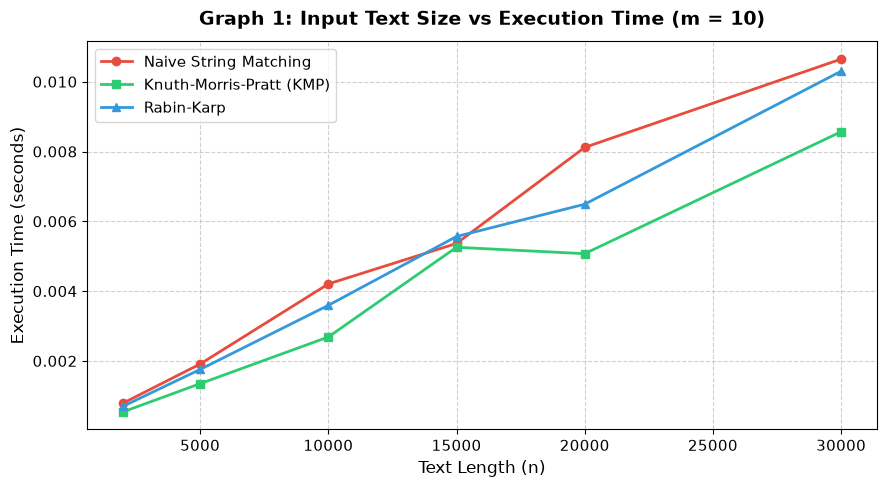
\includegraphics[width=0.88\textwidth]{plot_time_vs_n.png}
    \caption{Input Text Size ($n$) vs Execution Time ($m = 10$).}
    \label{fig:time_vs_n}
\end{figure}

\textbf{Analysis}:
As seen in Figure~\ref{fig:time_vs_n}, all three algorithms exhibit linear scaling with respect to input text length $n$ on random alphabets. KMP and Naive execute faster due to lighter per-character loop overhead compared to modular arithmetic in Python-level Rabin--Karp.

\subsection{Graph 2: Pattern Length vs Execution Time}
With a fixed text size ($n = 20,000$), the pattern length $m$ was varied from $5$ to $150$ characters.
\begin{figure}[H]
    \centering
    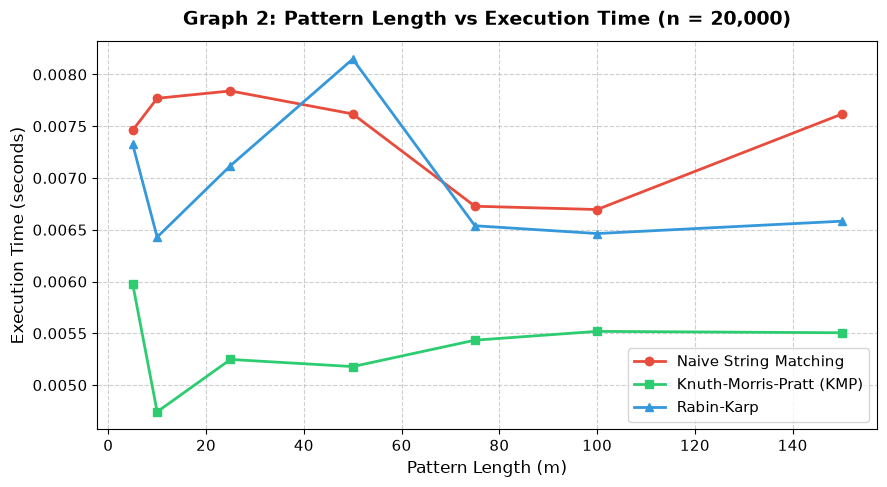
\includegraphics[width=0.88\textwidth]{plot_time_vs_m.png}
    \caption{Pattern Length ($m$) vs Execution Time ($n = 20,000$).}
    \label{fig:time_vs_m}
\end{figure}

\textbf{Analysis}:
Figure~\ref{fig:time_vs_m} illustrates that pattern length variation has negligible impact on KMP and Rabin--Karp search times because the search phase iterates through the text in $\mathcal{O}(n)$ steps. Preprocessing costs $\mathcal{O}(m)$ remain negligible for $m \ll n$.

\subsection{Graph 3: Input Size vs Number of Comparisons}
To clearly observe the theoretical advantage of KMP over Naive, text and pattern strings were generated over a binary alphabet $\Sigma = \{\text{'A'}, \text{'B'}\}$ with repeated prefixes ($P = \text{"ABABABABAB"}$), with text size $n$ varying from $1,000$ to $10,000$.
\begin{figure}[H]
    \centering
    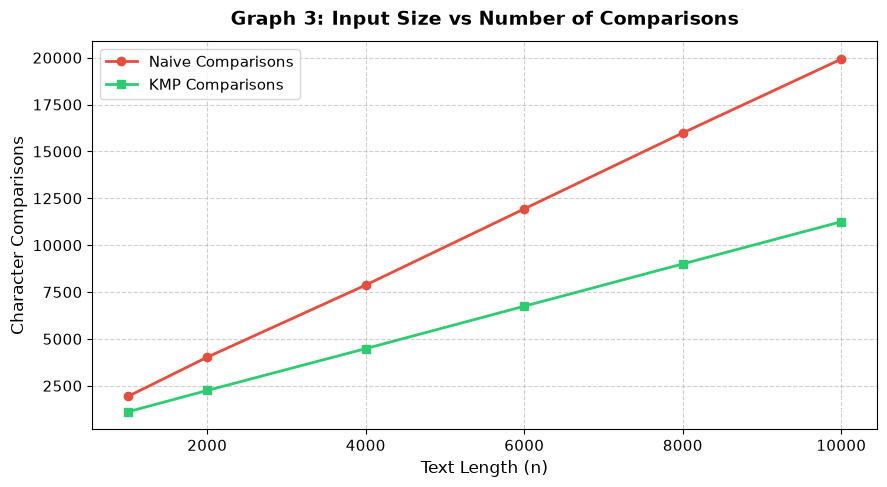
\includegraphics[width=0.88\textwidth]{plot_comp_vs_n.png}
    \caption{Input Size ($n$) vs Number of Character Comparisons (Repetitive Alphabet).}
    \label{fig:comp_vs_n}
\end{figure}

\textbf{Analysis}:
Figure~\ref{fig:comp_vs_n} demonstrates that on repetitive inputs with frequent partial matches, Naive requires significantly more comparisons due to shifting back to start each window. In contrast, KMP's LPS array prevents re-comparing matched prefixes, keeping comparisons strictly proportional to $n$.

% =========================================================================
% SUMMARY TABLE
% =========================================================================
\section{Summary and Conclusion}

\begin{table}[H]
\centering
\caption{Comprehensive Algorithmic Comparison}
\label{tab:comparison}
\begin{tabular}{@{}lccccc@{}}
\toprule
\textbf{Algorithm} & \textbf{Preprocessing} & \textbf{Matching Time} & \textbf{Space} & \textbf{Backtracking} & \textbf{Best Suited For} \\
\midrule
\textbf{Naive} & None ($0$) & $\mathcal{O}((n-m+1)m)$ & $\mathcal{O}(1)$ & Yes & Small texts, large alphabets \\
\textbf{KMP} & $\mathcal{O}(m)$ (LPS) & $\mathcal{O}(n)$ & $\mathcal{O}(m)$ & No & Repetitive text, small $\Sigma$ \\
\textbf{Rabin--Karp} & $\mathcal{O}(m)$ (Hash) & Avg: $\mathcal{O}(n+m)$, Worst: $\mathcal{O}(nm)$ & $\mathcal{O}(1)$ & No & Multi-pattern search, streaming \\
\bottomrule
\end{tabular}
\end{table}

\textbf{Final Remarks}:
\begin{enumerate}
    \item \textbf{Naive Matching} is simple to implement but performs poorly on repetitive data due to repeated character comparisons.
    \item \textbf{KMP Algorithm} achieves optimal deterministic $\mathcal{O}(n + m)$ runtime by using the LPS array to eliminate backtracking.
    \item \textbf{Rabin--Karp Algorithm} introduces rolling hashes, offering excellent average-case performance and a natural extension to 2D and multi-pattern matching problems.
\end{enumerate}

\end{document}
